\documentclass[a4paper]{article}
\usepackage[utf8]{inputenc}
\usepackage[polish]{babel}
\usepackage{polski}
\usepackage{parskip}

\usepackage[T1]{fontenc}
\usepackage{color}
\usepackage{listings}
\usepackage{indentfirst}
\usepackage[margin=0.9in]{geometry}
\usepackage{lmodern}
\usepackage{pdfpages}
\usepackage{pdflscape}
\usepackage{tabularx}

\setlength{\parindent}{25pt}
\setlength{\parskip}{1ex}
\definecolor{bluekeywords}{rgb}{0.13,0.13,1}
\definecolor{greencomments}{rgb}{0,0.5,0}
\definecolor{redstrings}{rgb}{0.9,0,0}
\pagestyle{plain}

% todo Nieprzewidziane koszty wyrazić w procentach np. +20 
% todo Poprawić tak, żeby tabele znajdowały się bezpośrednio w akapicie

\begin{document}


   	\title{\vspace{50mm}Skaner otoczenia na bazie robota mobilnego i sonaru}
	\author{Dorian Janiak, Marcin Ochman}
	\date{8 kwietnia 2015}

\maketitle

\newpage

\tableofcontents

\listoftables

\newpage

\section{Opis projektu}
Projekt realizowany jest w ramach kursu Roboty mobilne. W ramach projektu założyliśmy stworzenie małego robota mobilnego wyposażonego w sonar, który umożliwi rejestrowanie mapy otoczenia (jedynie horyzontalnie).
\subsection{Konstrukcja robota}
Sonar zostanie zrealizowany przy użyciu czujnika odległości zamontowanego na serwie. Serwo będzie zmieniało kąt czujnika, natomiast czujnik w tym czasie będzie wykonywał pomiary, które będą zapisywane w pamięci mikrokontrolera. Po wykonaniu pomiaru w danej pozycji robota dane zostaną wysłane do aplikacji komputerowej poprzez moduł Bluetooth. \newline 
Robot będzie typu jeżdżącego i nie będzie autonomiczny. Zastosujemy napęd na dwa koła, co pozwoli na obracanie robrota w miejscu. Aby zachować równowagę wyposażymy konstrukcję również w kulkę podpierającą. Sterowanie robotem odbywać się będzie przez Bluetooth z poziomu aplikacji komputerowej. Aplikacja komputerowa nie jest w tym wypadku optymalnym rozwiązaniem (lepszym byłby telefon np. z systemem Android), ponieważ zasięg Bluetooth jest stosunkowo niski, a więc użytkownik będzie zmuszony śledzić robota. Sterowanie robotem jednak nie jest głównym celem projektu.
\subsection{Cel projektu}
Cel projektu jest typowo zapoznawczy. Projekt ma umożliwić nam nauczenie się konstruowania robotów mobilnych, zmierzenie się z problemem doboru napędu i nim sterowania, obsługi komunikacji z urządzeniem zewnętrznym i zbieranie pomiarów z czujników zewnętrznych. Wynik naszej pracy posłuży nam oraz osobom pragnącym zabrać się za tworzenie własnych robotów. \newline
Założenie stworzenie sonaru jest o tyle istotne, że jest to poważny problem praktyczny. Prawie, że niezależnie od wyboru realizowanego problemu w dziedzinie robotów mobilnych robot powinien być w stanie zbierać informacje o otoczeniu. Omiatanie terenu przy pomocy jednego czujnika pozwoli mu przykładowo wybrać odpowiedni tor ruchu i ominąć duże przeszkody. 



\section{Plan pracy}

	
	W tym rozdziale zostanie opisany plan pracy nad robotem, który powinien doprowadzić do zbudowania robota oraz aplikacji przedstawionych w opisie projektu.
	
	\subsection{Kamienie milowe}
	
	Poniżej zostały przedstawione główne kroki, które należy wykonać aby zakończyć pracę nad projektem z oczekiwanymi rezultatami.
	
	\begin{table}[h]
	\centering
		\begin{tabularx}{0.8\linewidth}{|c|X|}
			\hline
			Lp. & Opis \\ \hline
			1  & Zbudowanie podwozia robota \\ \hline
			2  & Umieszczenie potrzebnej elektroniki - mikrokontroler, czujniki, serwomechanizm  \\ \hline
			3 & Oprogramowanie robota \\ \hline
			4 & Zakończenie pracy nad aplikacją na komputery osobiste do generowanie mapy otoczenia \\ \hline
			5 & Połączenie pracy robota i aplikacji \\ \hline
		\end{tabularx}
		\caption{Table opisująca poszczególne kamienie milowe}
	\end{table}
\subsection{Szczegółowy plan pracy}
	
	Poniżej został przedstawiony szczegółowy plan pracy nad projektem.
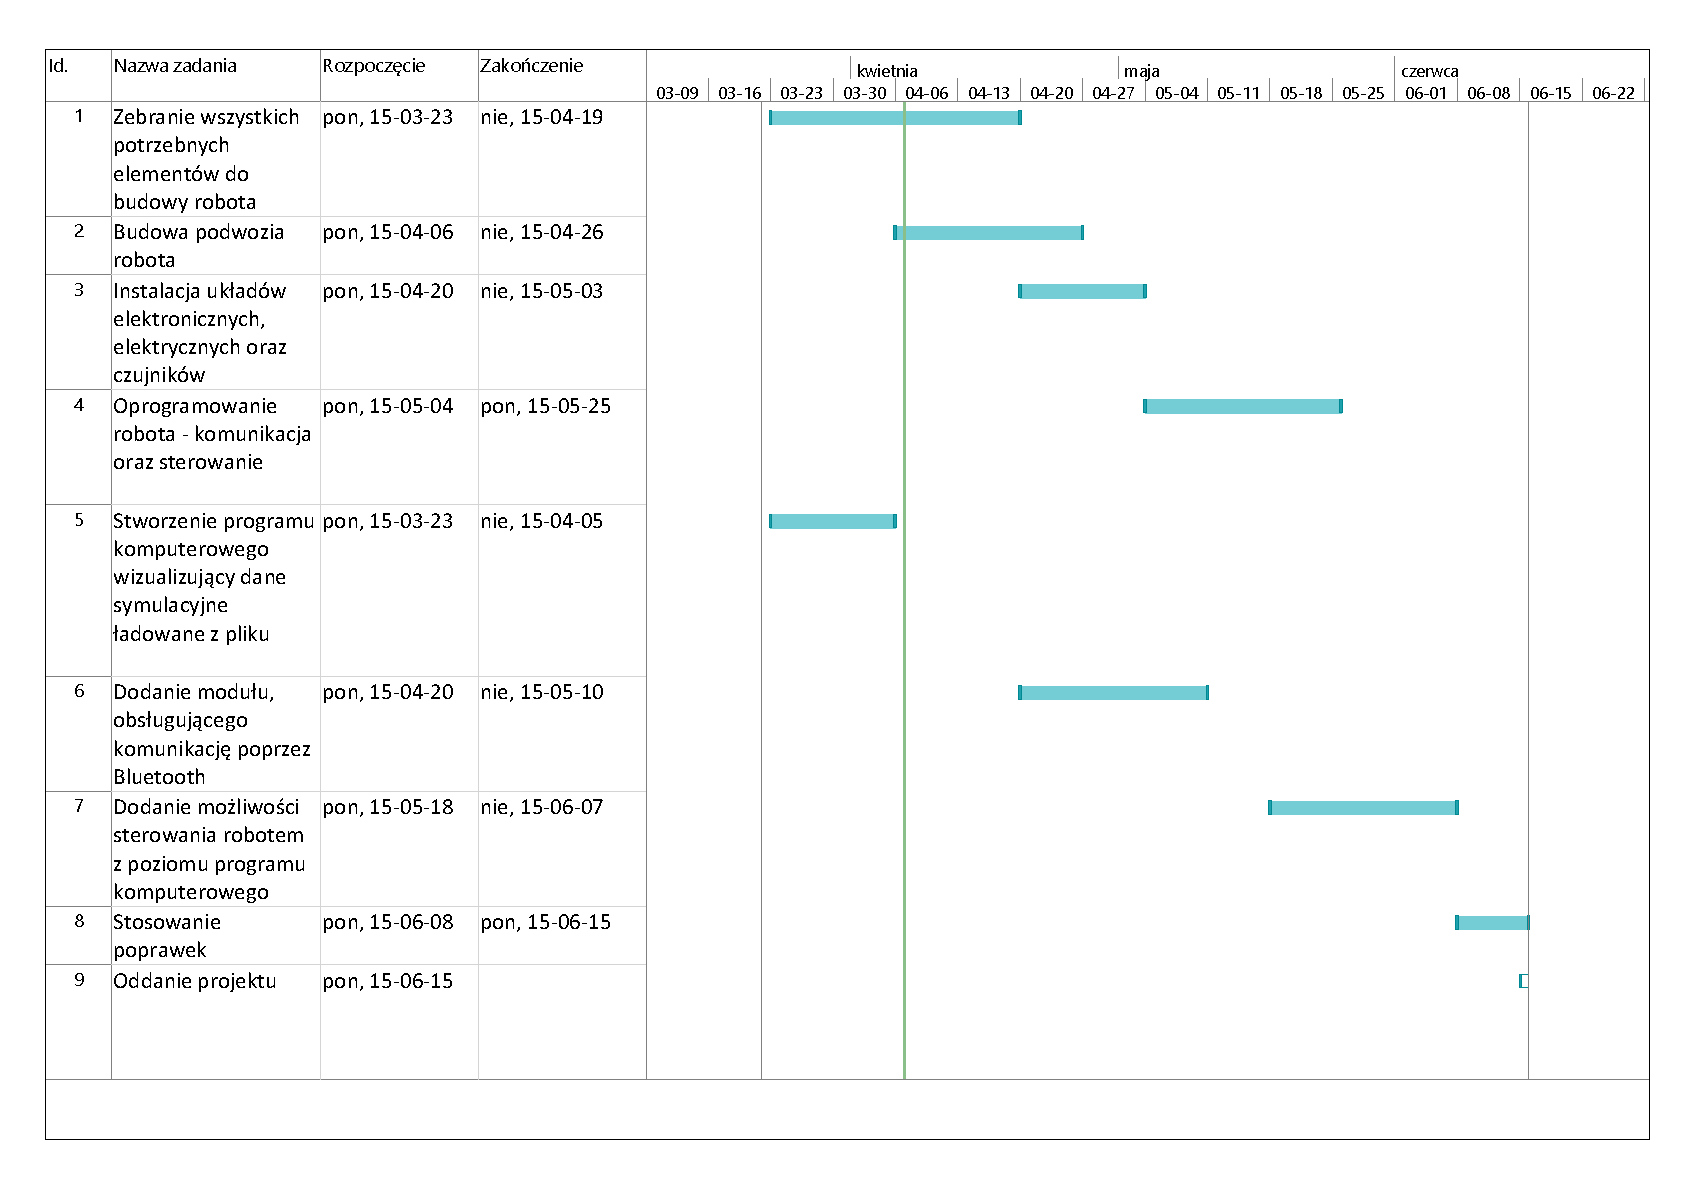
\includepdf[pages={1,2}, landscape]{MS_Project.pdf}
	
	



\section{Doręczenie}

Terminy i rodzaje dostarczanych w ramach projektu dokumentów oraz oprogramowania zostały przedstawione w Tabeli \ref{tabela_doreczenie}. Znalazły się również informacje o jawności.


\newcounter{rownumbercounter}
\newcommand\rownumber{\stepcounter{rownumbercounter}\arabic{rownumbercounter}}

\begin{table}[h]
	\centering
	\begin{tabularx}{\linewidth}{|c|X|c|X|c|}
		\hline 
		Nr & Nazwa & Termin & Postać & Jawność \\ \hline
		 \rownumber & Zbudowanie podwozia robota & 2 & sprzęt, dokumentacja & Grupa \\ \hline
		 \rownumber & Finalizacja pracy sprzętowej nad robotem & 3 & sprzęt, dokumentacja & Grupa \\ \hline
		 \rownumber & Oprogramowanie robota & 4 & oprogramowanie, dokumentacja & Grupa \\ \hline
		 \rownumber & Algorytm budowania mapy & 13 & oprogramowanie, dokumentacja & Grupa \\ \hline
		 \rownumber & Ukończenie prac nad aplikacją & 7 & oprogramowanie, dokumentacja & Grupa \\ \hline
		 \rownumber & Połączenie działania robota i aplikacji & 7,8 & oprogramowanie, sprzęt, dokumentacja & Publiczne \\ \hline
		 \rownumber & Raport końcowy & 9 & dokumentacja & Publiczna \\ \hline
		 
	\end{tabularx}
	\caption{Tabela doręczeń}
	\label{tabela_doreczenie}
\end{table}

\section{Budżet}
Ponieważ projekt ma charakter sprzętowy, a więc wymaga on kupna elementów. 

\begin{center}
\begin{tabular}{|c|c|}
\hline
\textbf{Element} & \textbf{Cena całkowita(zł)} \\ \hline\hline
Zestaw STM32 NUCLEO & 55 \\ \hline
Moduł Bluetooth HC-05 & 37 \\ \hline
Zestaw silników i kół z enkoderami Dagu RS034 & 110 \\ \hline
Serwo typu micro PowerHD & 16 \\ \hline
Kulka podporowa & 10 \\ \hline
Płytka PCB uniwersalna & 8 \\ \hline
Mostek H L298N & 11 \\ \hline
Pozostałe elementy zabezpieczające i zasilające & 30 \\ \hline
Nieprzewidziane koszty & 30 \\ \hline\hline
\textbf{Ogólny koszt:} & 307 \\ \hline

\end{tabular}
\end{center}


\section{Zarządzanie projektem i jego monitorowanie}
Ze względu na to, że projekt jest realizowany tylko przez 2 osoby, lider nie został wyznaczony. Tak mały zespół nie powinien mieć problemów komunikacyjnych. Realizować projekty będziemy częściowo zdalnie, jednak planujemy również regularnie się spotykać i wspólnie pracować nad projektem. Ustalenia będą powstawały w trakcie spotkań oraz w trakcie rozmów realizowanych na portalu facebook.com . Mimo, że jest to serwis społeczny, już od dłuższego czasu okazuje się, że nadaje się do komunikacji grup projektowych. Nasz projekt nie wymaga tworzenia grup użytkowników o różnych uprawnieniach, przydzielania zadań i tworzenia ich zestawień, a więc ten portal oraz umówione spotkania powinny wystarczyć. \newline
Współdzielić kod programów będziemy poprzez portal \textbf{github.com} . Nie zakładamy tajności projektu, a więc może być on udostępniony publicznie. \newline
Postępy monitorować będziemy na bieżąco poprzez porównanie aktualnych osiągnięć z harmonogramem. Kamienie milowe pozwolą nam ocenę ewentualnych opóźnień. Opóźnienia wymuszą na nas przyspieszenie prac lub ograniczenie założeń projektu.
\textsl{}


\section{Przydział zadań}
Ponieważ grupa składa się tylko z dwóch osób projekt w dużej mierze był realizowany wspólnie. Można  jednak wyróżnić część zadań, które miały być realizowane osobno. Podział prezentuje poniższa tabela (Tabela 4). Nakreśla ona wybór lidera danego zadania. Był on przede wszystkim odpowiedzialny za kontrolę czasu wykonania zadania.


\begin{table}[!htbp]
\begin{center}
\begin{tabular}{|c|c|c|}

\hline
\textbf{Nr} & \textbf{Nazwa zadania} & \textbf{Lider} \\ \hline\hline
Z1 & Zebranie wszystkich potrzebnych elementów do budowy robota & M. Ochman \\ \hline
Z2 & Budowa podwozia robota & M. Ochman \\ \hline
Z3 & Instalacja układów elektronicznych, elektrycznych oraz czujników & M.Ochman \\ \hline
Z4 & Oprogramowanie robota - komunikacja oraz sterowanie & M.Ochman \\ \hline
Z5 &Stworzenie programu komputerowego wizualizujący dane symulacyjne ładowane z pliku & D. Janiak \\ \hline
Z6 & Dodanie modułu, obsługującego komunikację poprzez Bluetooth & D.Janiak \\ \hline
Z7 & Dodanie możliwości sterowania robotem z poziomu programu komputerowego & D.Janiak \\ \hline
Z8 & Stosowanie poprawek & D.Janiak \\ \hline


\end{tabular}
\caption{Podział zadań w grupie}
\end{center}
\end{table}

W skład grupy wchodziły osoby:
\begin{description}
\item[Marcin Ochman] - student AiR. Wybrał specjalność Robotyka, ponieważ interesuje się zarówno komputerami, elektroniką oraz nowinkami technicznymi.
	Jego głównym atutem jest umiejętność programowania w różnych językach takich jak C, C++, C\#, Python, SQL. 
	Swoje doświadczenie zdobywa zarówno na uczelni oraz pracując w firmie Vulcan.	
\item[Dorian Janiak] - Pisze od kilku lat programy w językach C++/C. Podejmował się również pracy z takimi językami jak Python, Matlab czy QML. Obecnie pracuje jako programista C++. Jego głównym zainteresowaniem jest grafika 3D (używał OpenGL i GLSL, zna podstawy RayTracingu, posługuje się programem Blender 3D). Ukończył kurs języka niemieckiego na poziomie B2.
\end{description}



\end{document}
